\documentclass[a4paper]{article}

\usepackage{lgrind}
\usepackage{graphicx}
\usepackage{hyperref}

\author{Paul van der Walt\\\url{paul@denknerd.org}}
\date{\today}
\title{Parallel Algorithms: Eratosthenes' Sieve}

\begin{document}
\maketitle
\begin{abstract}
    In this report the findings are presented after benchmarking the Dutch
    supercomputer Huygens and a personal computer. The Sieve of Eratosthenes is
    then implemented in sequence and parallel (including a number of performance
    improvements), and tested on Huygens and a
    personal computer. 
\end{abstract}
\tableofcontents

\section{Introduction}

This report documents the use of BSP-style\cite{BSP} parallel programming to
find primes in parallel, using Eratosthenes' method. 

The so-called sieve of Eratosthenes is an old and unsophisticated method for
finding all primes up to a given number $N$, which lends itself quite nicely to
parallelisation. The idea is roughly as follows: start with the lowest known
prime $i$ (given: $i \leftarrow 2$ in the first iteration) and cross all
multiples of $i$ out of your list of potential primes, which starts off with all
natural numbers 1\ldots$N$. While $i$ is less than $N$, repeat. The next lowest
known prime is the smallest number which hasn't been crossed off the list yet.
More information about Eratosthenes' prime sieve can be found in Section
\ref{sec:sieve}. 

Secondly, we take a look at benchmarking BSP computers and the performance
measured when testing on Huygens\cite{sarahuygens}, the Dutch national
supercomputer, and on a recent MacBook. Specifically, the benchmark is aimed at
parallel computers, measuring not only computation speed, but also
synchronisation time and communication speed. 



\section{Prime Sieve}\label{sec:sieve}

\subsection{Description}

To quickly recap, Eratosthenes' method finds all prime numbers less than or
equal to $n$. There are a number of obvious and less
obvious improvements which can be made on this algorithm, but at its most basic
form it is as follows. 

\begin{enumerate}
    \item Create a list of consecutive integers from two to $n$: (2, 3, 4, ...,
        $n$).
    \item Initially, let $p$ equal 2, the first prime number.
    \item Strike from the list all multiples of $p$ less than or equal to $n$.
        ($2p, 3p, 4p$, etc.)
    \item Find the first number remaining on the list after $p$ (this number is
        the next prime); replace $p$ with this number.
    \item Repeat steps 3 and 4 until $p^2$ is greater than $n$.
    \item All the remaining numbers in the list are prime.
\end{enumerate}

This algorithm will be assumed correct (proof is outside the scope of this
report). One of the
first optimisations is that crossing off can begin at $p^2$ since all smaller
multiples of $p$ will already have been crossed off in earlier iterations. The
time complexity after this optimisation is $O(n \log \log n)$ \cite{pp}. Another
optimisation one could implement is to not make a list of all $n$ numbers, but
leave out all even numbers, since these are known to be non-prime. This will
save half the necessary memory, but asymptotically this makes no difference for
memory requirements in the RAM model. 

The sequential implementation can be found in Appendix \ref{app:seq}, and
follows this algorithm closely. Since this program was only used as a means to
implementing a working sequential sieve, the time results will be omitted. 

\subsection{Data distribution}

As a result of the BSP model's non-shared memory assumption,  finding a parallel
implementation of our algorithm starts with deciding on a good data
distribution. The consideration is that most of the work the algorithm does is
crossing off numbers, therefore, we must distribute such that the crossing off
of numbers is as evenly distributed over processors as possible. The first idea
is then to use a so-called block distribution, where given $P$ processors and
$N$ values, we give the each processor $\lceil N/P \rceil$ values, until the
last processor, which we give $\lfloor N/P \rfloor$ values. This way, we can
broadcast the smallest prime found, each processor can independently cross
multiples off and find it's local minimum prime, and let $P(0)$ calculate the
global minimum prime, and repeat. For more on the BSP model and data
distributions, see \cite{biss}.

\subsection{The parallel algorithm}

More formally, the algorithm becomes as follows. In common BSP style, the
algorithm is parameterised by the current processor ID $s$. The functions
minidx(), maxidx() and local() are used for keeping track of indices in the
array, since it has been split into blocks over the processors. Min and maxidx
give the minimum and maximum number stored on a given processor, and local gives
the local index of a number on a processor (this is found by calculating the
argument modulo $\lceil N/P \rceil$, roughly). See Appendix \ref{app:par} for
implementational details. 

\begin{enumerate}
    \item Initialise a list $A$ minidx($s$) .. maxidx($s$), all \texttt{true}.
    \item If $s=0$ then $A_1 \leftarrow $\texttt{false} (we know 1 isn't prime).
    \item Set $k\leftarrow 2$ (2 is our largest prime to start off with).
    \item While $k^2 \le n$ \textbf{do}
        \begin{enumerate}
            \item For $i \in {k, 2 k, \cdots }$ set $A_{\textnormal{local}(i)} \leftarrow
                $\texttt{false} (eliminate multiples of $k$ locally).
            \item Find $m_s \leftarrow \displaystyle \textnormal{argmin}_{i}
                (A_i = \texttt{false})$ (local next prime).
            \item If $s=0$ then read all $m_i$ and select minimum (collect local
                next primes).
            \item Broadcast as $k$ (global next prime).
        \end{enumerate}
    \item \textbf{od}
\end{enumerate}

\subsection{Complexity}

\ldots

\section{Performance}

\subsection{Timed results}
Next we put our algorithms to the test. We hope to see a marked improvement over
the sequential (read: $P=1$) implementation, since the complexity is much better
when $P$ increases. 

The obtained results can be seen in Table \ref{tbl:results}. 

\begin{table}
    \centering
    \begin{tabular}{c|cccccc}
        Computer & $P=1$ & $P=2$ & $P=4$& $P=8$& $P=16$& $P=32$    \\
        \hline
        Huygens & 20.36 & 10.87 & 5.54 & 2.96 & 1.91 & 11.28 \\
        MacBook & 12.14 &  7.60 & 7.88 & 8.40 &11.16 & 30.04 \\
        \hline
    \end{tabular}
    \caption{The results when running sequential and parallel implementations of
    the Sieve of Eratosthenes. In all cases, $N=10^8$ and unit of time is
    seconds. }
    \label{tbl:results}
\end{table}


\subsection{Analysis of results}

A number of things are clear when we look at the results of Table
\ref{tbl:results}. First of all, we see that the laptop indeed outperforms
Huygens when using a single core, which is also seen in Section \ref{sec:bench}
where the raw computational rate $r$ is measured to be higher on the laptop. The
most likely cause for this is that when running on the laptop, all other
processes can be given lower priority, enabling the sieve to use all available
processor power. On Huygens, however, nodes are shared, and therefore we are not
the sole users of a given node. 

When we start increasing $P$ we see the profit from parallelising the algorithm.
The running time roughly halves, as expected, when running on 2 cores, and for
the MacBook, this is when maximal performance is achieved. This is because the
MacBook has a dual-core processor, so setting $P=2$ is making optimal use of the
resources. On Huygens, however, nodes have 16 cores each, which is why we see a
continuing decrease in running time until $P=16$. The sudden increase at $P=32$
is as a result of using 2 nodes with 16 cores each; now the communication has to
cross an intermediary network and isn't local any more. 

On the MacBook, the reason for the time increase is different: all threads are
still local, but since there are only 2 cores, creating more threads only adds
to the overhead which BSP has to administer, and doesn't off a performance
improvement. 

These results are all consistent with our theoretical analysis of the algorithm,
namely that the performance will increase linearly with the number of processors
available, assuming communication cost doesn't dominate, which is what we see in
the case of $P=32$ on Huygens. 

\section{Benchmarks}\label{sec:bench}

The two computers tested in this section, as already mentioned, are a recent
MacBook\footnote{Core2Duo 2.4Ghz with 4GB memory.} and Huygens, the national
supercomputer. Of course we didn't do the benchmark on all the processors of Huygens,
as there are in the order of three thousand of them, but only on 1 and 2 nodes
(each node has 16 cores). 

The benchmark that has been done is the one included in BSPedupack which can be
found at \cite{edupack}, referred to as \texttt{bspbench.c}. The results are
presented in Figures \ref{fig:bench-huy-put-p2} to
\ref{fig:bench-laptop-get-p56}. In all these figures, the horizontal axis
represents the value of the $h$-relation, in other words, how many data words
are communicated in the communication superstep, and the vertical axis
represents the time (in flops) taken for the communication superstep.
Furthermore the well-known meanings of $r$, $g$ and $l$ hold, namely computation
rate, communication cost per data word in flops and sync time in flops,
respectively. 

\subsection{Original benchmark}
\begin{figure}[h]
    \begin{center}
        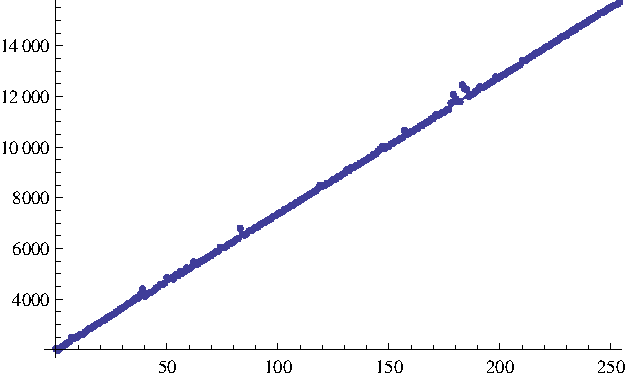
\includegraphics{img/bench-huy-put-p2.pdf}
    \end{center}
    \caption{Benchmark results on Huygens with $P$=2; the benchmark bottom line
    was $r=$ 194.357 Mflop/s, $g=$ 54.2, $l=$ 1986.4}
    \label{fig:bench-huy-put-p2}
\end{figure}

\begin{figure}[h]
    \begin{center}
        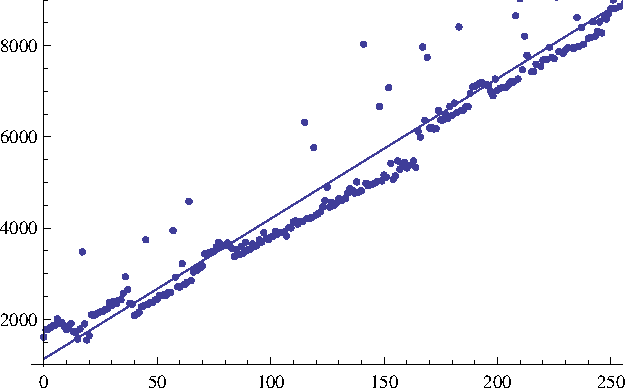
\includegraphics{img/bench-laptop-put.pdf}
    \end{center}
    \caption{Benchmark results on MacBook with $P$=2; bottom line was  $r=$
    399.853 Mflop/s, $g=$ 30.9, $l=$ 1112.4 }
    \label{fig:bench-laptop-put-p2}
\end{figure}

In figures \ref{fig:bench-huy-put-p2} and \ref{fig:bench-laptop-put-p2} we see
the results of running the plain benchmark on Huygens and the laptop.
Interestingly enough, the laptop seems to perform better than Huygens in all
respects. The only reason we can give for this is that the shared cores on
Huygens are a lot more overworked than the laptop when it is doing nothing else
other than running the benchmark. In a sense this is therefore an unfair
comparison.

Note that on Huygens we used 1 node, which means the communication would
probably be cheaper than if we were to do the same benchmark, but distribute it
over 2 nodes, so the communication has to leave the node as opposed to being
local, as it would have been in Figure  \ref{fig:bench-huy-put-p2}. 

We see predictable and expected linear behaviour on Huygens, but the laptop
results are a
lot more noisy. We attribute this to the fact that other processes such as the
graphical user interface are running which generate unpredictable performance
hits. These observations also hold on the get-versions of these 2 tests.

\begin{figure}[h]
    \begin{center}
        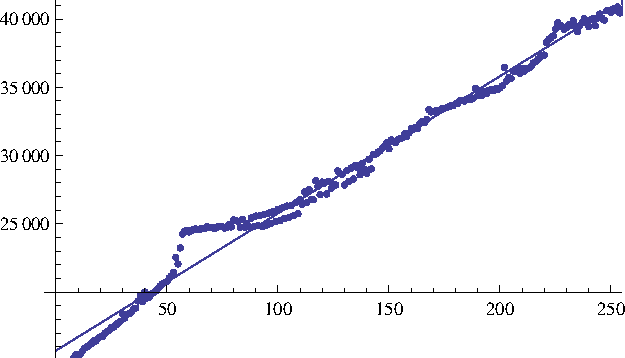
\includegraphics{img/bench-huy-put-p2-dist.pdf}
    \end{center}
    \caption{The same test as in Figure \ref{fig:bench-huy-put-p2}, but then
    instead of 2 processes on one node, we tried 2 processes on 2 nodes. The
    bottom line becomes $r=$ 195.648 Mflop/s, $g=$ 100.2, $l=$ 15770.4}
    \label{fig:bench-huy-put-p2-dist}
\end{figure}

The results shown in Figure \ref{fig:bench-huy-put-p2-dist} are when we select 2
distinct nodes on Huygens. We indeed see a marked increase in communication cost
$g$ and synchronisation cost $l$. As we would expect, the computational rate $r$
is basically unaffected by this change, as the work needing to be done locally
is the same as before. 

Since here we are forcing network communication, the performance becomes more
interesting to analyse. Where the local version (Figure
\ref{fig:bench-huy-put-p2}) has a very straight performance ``curve'', we now
observe a peak and some waviness. The waviness is attributed to other network
communication outside of our control which will affect the speed with which our
packets reach their destination; the peak is possibly the point at which the
underlying layer decides to switch to another, more high-volume, communication
scheme. The latter point is, however, guesswork, without knowing more about our
platform. 

\subsection{Changing to \texttt{get}s}
Now we change puts into gets in the benchmark algorithm. The hypothesis is that
getting is more expensive than putting, since a put is passive with respect to
the receiver, whereas when getting both processors have to work. See figures
\ref{fig:bench-huy-get-p2} to \ref{fig:bench-huy-get-p2-dist}. 

\begin{figure}[h]
    \begin{center}
        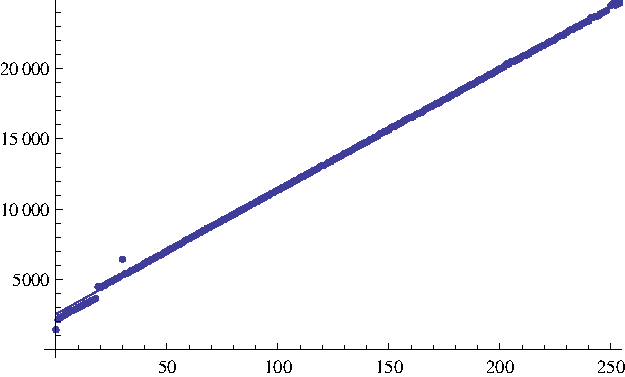
\includegraphics{img/bench-huy-get-p2.pdf}
    \end{center}
    \caption{Having changed \texttt{put}s into \texttt{get}s we measure again on
    Huygens with $P=2$. Bottom line: $r=$ 191.062 Mflop/s, $g=$ 87.2, $l=$ 2574.6}
    \label{fig:bench-huy-get-p2}
\end{figure}

\begin{figure}[h]
    \begin{center}
        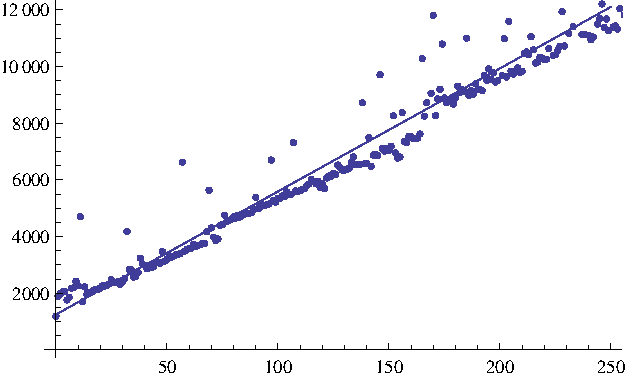
\includegraphics{img/bench-laptop-get.pdf}
    \end{center}
    \caption{MacBook with $P=2$. Bottom line: $r=$ 389.348 Mflop/s, $g=$ 43.5, $l=$ 1240.1}
    \label{fig:bench-laptop-get-p2}
\end{figure}

Comparing \ref{fig:bench-huy-get-p2} and \ref{fig:bench-laptop-get-p2} to the
corresponding figures in the previous section, we indeed see a marked increase
in communication cost (note: not in synchronisation cost) on Huygens. Surprisingly enough, on the laptop, this
increase is not so great on the laptop. We expect and observe the
synchronisation time to be comparable with puts and gets, since this change
shouldn't affect the synchronisation steps. 

\begin{figure}[h]
    \begin{center}
        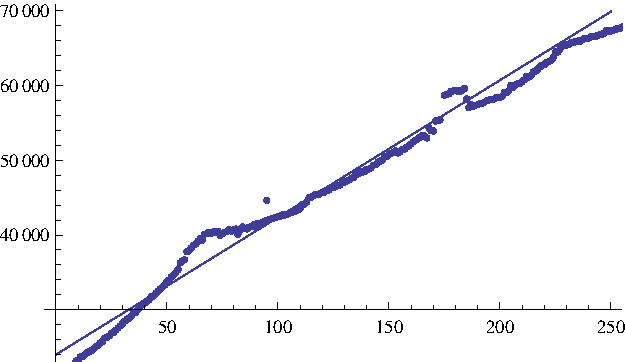
\includegraphics{img/bench-huy-get-p2-dist.pdf}
    \end{center}
    \caption{The same test as in Figure \ref{fig:bench-huy-get-p2}, but then
    instead of 2 processes on one node, we tried 2 processes on 2 nodes. The
    bottom line becomes $r=$ 194.498 Mflop/s, $g=$ 182.3, $l=$ 24222.0}
    \label{fig:bench-huy-get-p2-dist}
\end{figure}

Once again, we try forcing the benchmark to run on 2 distinct nodes on Huygens
(see Figure \ref{fig:bench-huy-get-p2-dist}). Again the computation rate $r$ is
the same, communication cost $g$ is significantly increased, but in this case,
also $l$ suffers, increasing by nearly a factor of 2. We cannot give an
explanation for this, and attribute it to incidental load on the shared node
being used. Note that this is plausible seeing the entire benchmark runs in
about 20 seconds, which will never give a very accurate picture of a computers
average performance. 

We also see not 1, but at least 2 discernible peaks in the curve. Once again the
conjecture is that the communication schemes used switch at these points. 

As a last effort at producing more interesting results, we run the benchmark on
the laptop with $P=56$. This isn't done on Huygens since it will be a waste of
resources and will probably have to wait a long time in the queue. See Figure
\ref{fig:bench-laptop-get-p56}. The results here speak for themselves: the
computation rate $r$ is still independent of the configuration, but the
communication cost and specifically synchronisation time skyrocket. The reasons
for this are obvious: namely, communication becomes more costly when the
underlying BSP layer has to manage more and more processors, and the
synchronisation cost is hypothesised to be $\omega(n)$ (i.e. at least linearly increasing in
the number of processors used, $N$). 

\begin{figure}[h]
    \begin{center}
        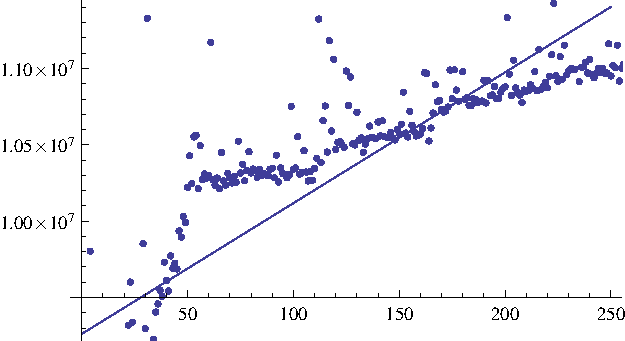
\includegraphics{img/bench-laptop-get-p56.pdf}
    \end{center}
    \caption{Test on the MacBook with $P=56$, using \texttt{get}s. Bottom line
    now becomes $r=$ 445.799 Mflop/s, $g=$ 4201.9, $l=$ 10037639.0}
    \label{fig:bench-laptop-get-p56}
\end{figure}

Interestingly we also see a sharp increase in communication time before $h=56$,
where after that point the time levels out to become linear. This is logical,
since before $P=56$, not all processors are being communicated with, so the
communication superstep takes much longer each time an extra processor is talked
to. After all the processors have been communicated with (i.e. $h>56$) BSP is
smart enough to bundle communication to a given processor, so that the
communication time increases linearly in $h$. 



\appendix
\section{Sequential sieve code}\label{app:seq}

\lgrindfile{../seq/sieve.lg}

\section{Parallel sieve code}\label{app:par}

\lgrindfile{../par/bspsieve.lg}


\begin{thebibliography}{99}
    \bibitem[BSP]{BSP} \url{http://www.bsp-worldwide.org}, homepage of the BSP
        association. 
    \bibitem[SHuy]{sarahuygens}
        \url{https://subtrac.sara.nl/userdoc/wiki/huygens/description},
        information page on the Huygens supercomputer. 
    \bibitem[BSPep]{edupack}
        \url{http://www.staff.science.uu.nl/~bisse101/Software/software.html}, homepage of BSPedupack, an education set of sample code for the
        BSP library. 
    \bibitem[Prit87]{pp} Pritchard, Paul, "Linear prime-number sieves: a family tree," Sci. Comput. Programming 9:1 (1987), pp. 17–35.
    \bibitem[Biss04]{biss} Rob H. Bisseling, Parallel Scientific Computation: A Structured Approach using BSP and MPI, Oxford University Press, March 2004. ISBN 978-0-19-852939-2
\end{thebibliography}

\end{document}
